\section{第6問：少数三角形による画像近似と美しさの代理目的}
\label{sec:q06}

\subsection{狙いと実験の位置づけ}
画像を多数の画素として記憶する代わりに，少数の三角形の組合せとして表す．本実験では，「三角形を増やして誤差を減らす」だけでなく，輪郭の保持，色のまとまり，ノイズへの頑健性，表現の簡潔さの間にどのような関係があるかを調べた．位置・色・描画順を遺伝子とする間接表現は，Bergらの進化的画像表現とも共通する考え方である\footnote{J. Berg et al., \emph{Evolved Art with Transparent, Overlapping, and Geometric Shapes}, NAIS 2019, \url{https://arxiv.org/abs/1904.06110}．}．実装は独自に作成した．

問題例として，著作権や撮影条件の影響を避けた自作の64\,$\times$\,64 RGB画像3種類を用いた．風景は山・雪・水面などの明瞭な境界，果実は曲線と陰影，勾配画像は連続的な色変化と小さな円形境界を持つ．このように性質を分けることで，単一の絵で得た成功を画像一般の性質と取り違えないようにした．

\begin{figure*}[t]
\centering
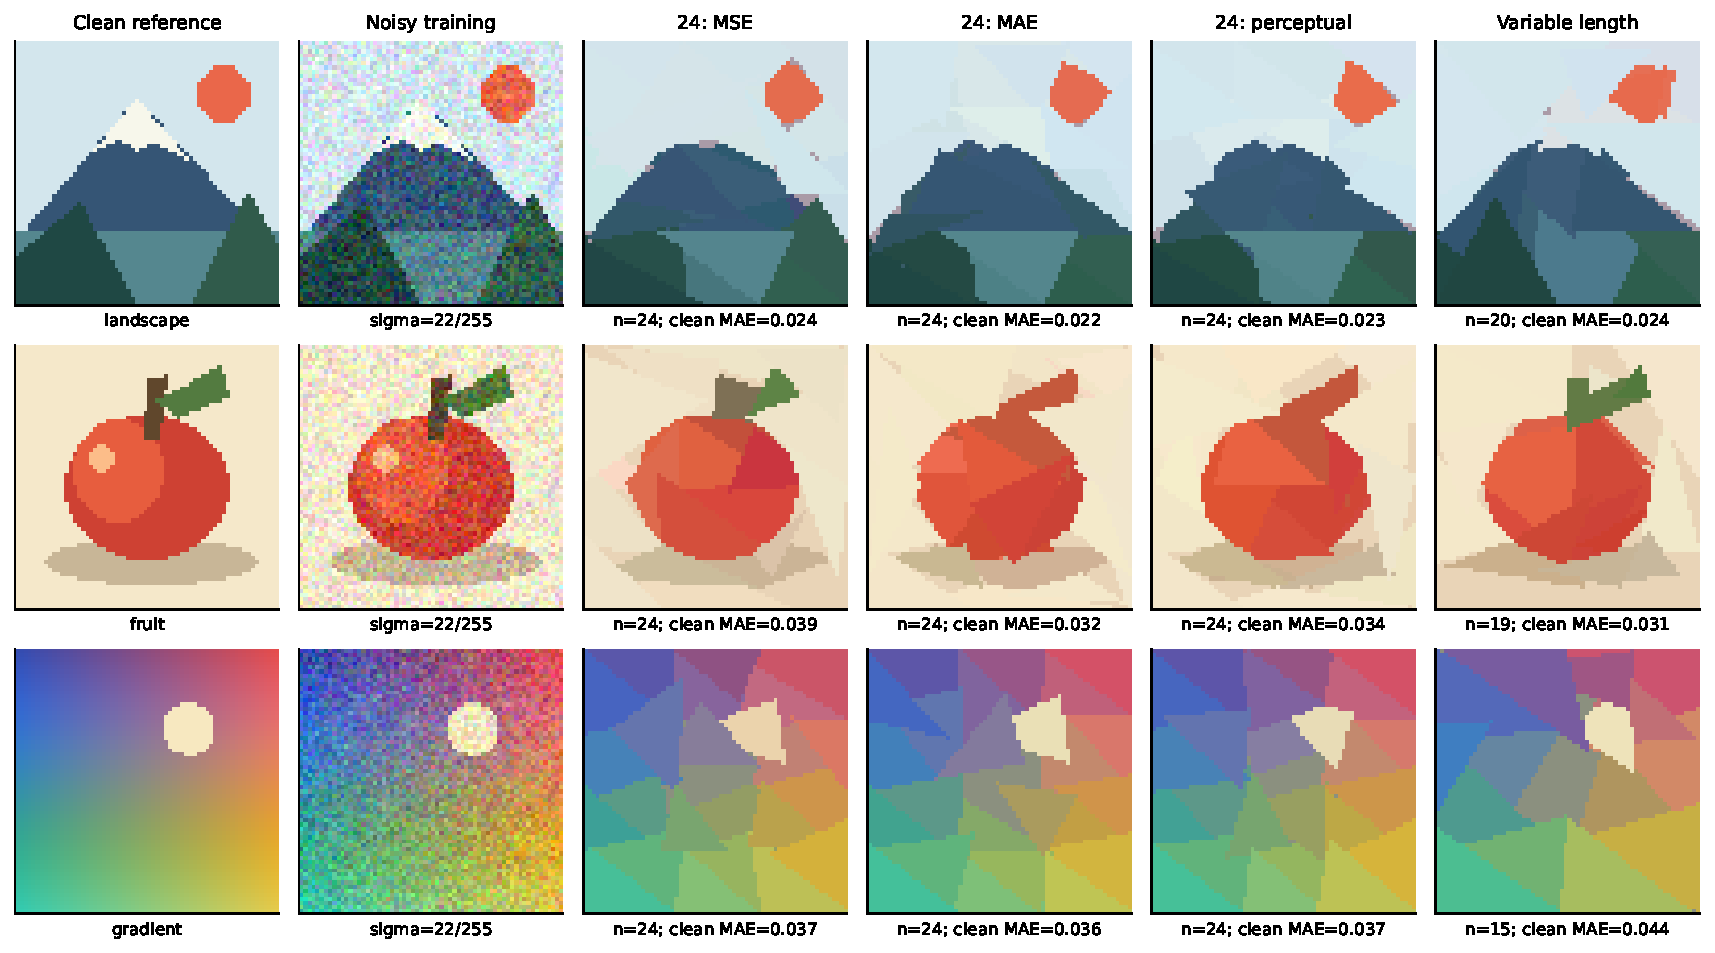
\includegraphics[width=\textwidth]{06/results/reconstructions.pdf}
\caption{第6問の入力と実測結果．各行は自作の風景・果実・勾配画像．左から原画像，ノイズを含む学習画像，24三角形のMSE・MAE・知覚代理目的，可変長表現．再現画像は事前に固定した乱数seed 0の結果であり，5回から見栄えの良いものを選んでいない．表示するclean MAEは最適化時に使っていない原画像に対する誤差である．}
\label{fig:q06_montage}
\end{figure*}

\begin{figure*}[t]
\centering
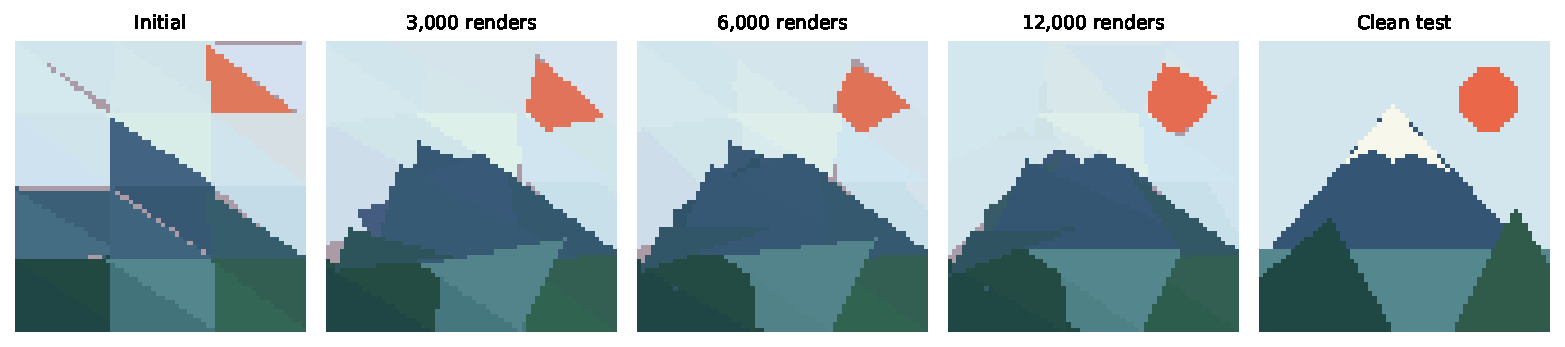
\includegraphics[width=\textwidth]{06/results/progression.pdf}
\caption{ノイズ風景・24三角形・MAE・seed 0の進化過程．初期の格子状の面が，3,000，6,000，12,000描画とともに主要境界を説明する形へ変化する．右端は探索に使っていないノイズなし参照．}
\label{fig:q06_progression}
\end{figure*}

\subsection{遺伝子型と探索手続き}
個体は順序付きリスト
\begin{equation}
 G=(t_1,\ldots,t_n),\qquad
 t_i=(x_1,y_1,x_2,y_2,x_3,y_3,r,g,b)
\end{equation}
とした．三角形は不透明であり，後に描くものが前のものを覆う．座標とRGB値を連続変数として持ち，評価時には座標を整数画素に丸める．背景は学習画像の各色成分の中央値に固定した．これは半透明色の重ね合わせによる描画とは異なり，面と輪郭の構成を明瞭に比較するための設計である．

初期集団は格子を三角分割した配置に小さい乱数摂動を与え，領域内の学習画素の平均値（MSE）または中央値（その他）で初期色を決めた．さらに突然変異の一部で同じ色推定を行う．したがって，画像の情報を初期化と提案に利用するハイブリッドGAである．目的関数の比較は，対応する平均値／中央値の色推定も組み合わせた設定間の比較であり，損失関数だけの効果を分離する実験ではない．この工夫は探索開始時から粗い色面を確保するが，学習画像へのアクセスを追加で行うため，純粋な無情報探索との優劣を主張するものではない．

基本の集団サイズは12とし，3個体のトーナメント選択，確率0.15の一点交叉，突然変異を使う．交叉は三角形リストの前半と後半を交換する．突然変異では頂点の移動，三角形の平行移動，色変更，描画順の交換を行う．新しい子1個体を評価し，集団の最悪個体より良く，かつ同じ目的値の重複でない場合に置換する$(\mu+1)$型の定常状態GAである．最良値は悪化しないが，大域最適性は保証しない．

可変長版は12三角形で初期化し，長さを2--48の範囲とした．挿入では残差が大きい場所を確率的に選んで新しい三角形を追加し，削除では1個の三角形を除く．通常の挿入分岐は8\%，削除分岐は7\%であり，長さの上下限では許された分岐のみを使う．新しい三角形の追加が必ず採択されるわけではなく，誤差改善が複雑さの費用に見合う必要がある．

\subsection{適合度と「美しさ」の定義}
RGB値を$[0,1]$に正規化し，基本目的としてMSEとMAEを比較した．さらに，色面の誤差と輪郭の誤差を組み合わせる次の代理目的を設計した．
\begin{align}
 L_{\rm p}&=\frac{\sum_{p}w_p\,d_p}{\sum_p w_p}
              +0.35\,D_{\rm edge},\\
 d_p&=\frac{1}{3}\sum_c |I_{p,c}-T_{p,c}|,\\
 w_p&=1+3\left(\overline{|\Delta_xT_p|}
                         +\overline{|\Delta_yT_p|}\right).
\end{align}
ここで$I$は描画画像，$T$は学習画像であり，$\Delta$は隣接画素の前進差分，横線はRGB平均を表す．$D_{\rm edge}$は$x,y$各方向について計算したRGB差分のMAEの平均である．画像端で存在しない差分は画素重みへの寄与を0とした．

可変長版では$L_{\rm p}+\lambda n$を最小化する．標準値は$\lambda=0.0007$とし，風景のノイズなし条件では$0$と$0.0015$も比較した．本実験での「美しさ」は，少ない面で主要な色と境界を説明するという操作的定義である．人間の主観評価を実施していないため，この目的値の低下をそのまま人間にとって美しいことの証明とはしない．

\subsection{比較条件と学習・テストの区別}
主要実験は，3画像$\times$学習画像の2条件（原画像／ノイズ画像）$\times$6設定$\times$5 seedの180試行である．6設定はMAEで8・24・48三角形，24三角形のMSE，24三角形の知覚代理目的，知覚代理目的の可変長版とした．ノイズは0--255スケールで標準偏差22の独立な正規乱数とし，範囲外をクリップした．全探索でseed 0--4を使い，学習ノイズはseed 20261117に固定した．

さらに，ノイズなし風景で集団サイズ4・36，画像に基づく色の再推定を無効化した変異，可変長の罰則2条件を各5回比較した．合計205試行，1試行12,000候補，総計2,460,000回の描画評価である．初期集団の評価もこの回数に含めた．三角形数によって1回の描画の費用は異なるため，描画数を揃えた比較に加え，実時間もJSONに記録した．

評価を終えた遺伝子を固定し，(i)ノイズなし原画像，(ii)別seed 918211のノイズ画像，(iii)太陽位置などを少し変えた類似画像，(iv)別種類の画像に対してMAE・MSE・PSNR・輪郭誤差を計算した．ノイズ学習条件では(i)の原画像を探索関数に渡しておらず，ノイズ除去の評価に使える．原画像で学習する条件では(i)が学習対象そのものなので，clean MAEは学習時の再構成誤差である．(ii)--(iv)は両学習条件とも探索に使わない．ただし，本方式は画像1枚ごとの最適化であり，画像一般を入力から変換する学習済みモデルではない．類似画像テストは固定した表現の変化への感度を調べるもので，別画像にも自動で適応できるという意味の汎化実験とは区別する．

\begin{figure}[t]
\centering
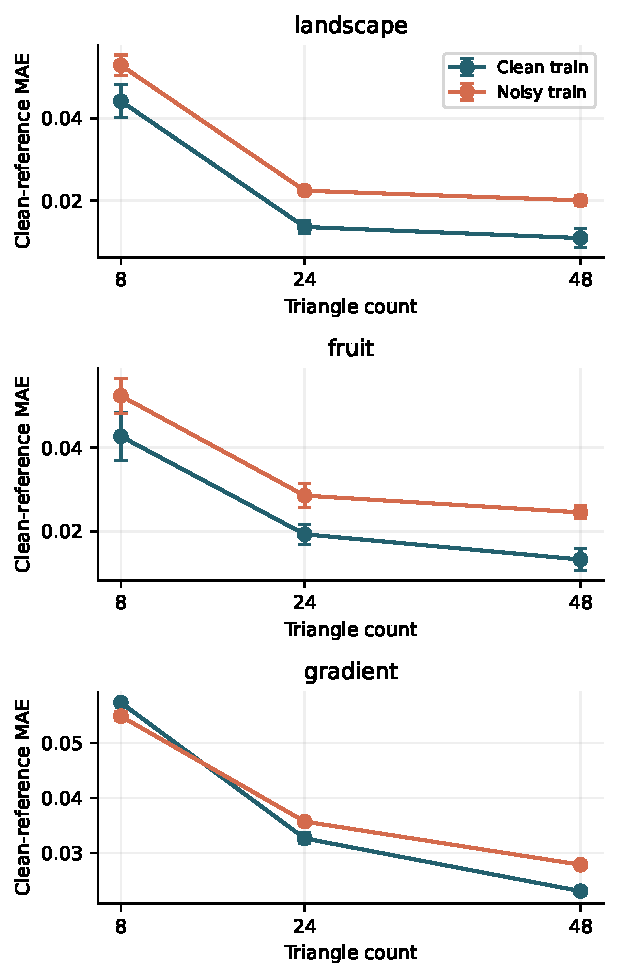
\includegraphics[width=\linewidth]{06/results/complexity.pdf}
\caption{三角形数とノイズなし参照へのMAE．原画像で学習した曲線は再構成誤差，ノイズ画像で学習した曲線は未使用の原画像への誤差である．点は5 seedの平均，誤差棒は標本標準偏差．同じ12,000描画でも，個体の次元と1描画あたりの費用は異なる．}
\label{fig:q06_complexity}
\end{figure}

\begin{table}[t]
\centering
\caption{ノイズ画像で最適化した結果の5 seed平均．評価先はノイズなし原画像．全条件の標準偏差と他の指標は公開CSVに収録した．}
\label{tab:q06_result}
\small
\begin{tabular}{llrrr}
\toprule
画像 & 適合度 & $n$ & clean MAE & edge MAE \\
\midrule
風景 & MSE & 24.0 & 0.028 & 0.015 \\
風景 & MAE & 24.0 & 0.022 & 0.016 \\
風景 & 知覚代理 & 24.0 & 0.024 & 0.016 \\
風景 & 可変長 & 18.8 & 0.024 & 0.015 \\
\midrule
果実 & MSE & 24.0 & 0.037 & 0.016 \\
果実 & MAE & 24.0 & 0.029 & 0.018 \\
果実 & 知覚代理 & 24.0 & 0.031 & 0.016 \\
果実 & 可変長 & 16.2 & 0.033 & 0.016 \\
\midrule
勾配 & MSE & 24.0 & 0.037 & 0.014 \\
勾配 & MAE & 24.0 & 0.036 & 0.014 \\
勾配 & 知覚代理 & 24.0 & 0.036 & 0.014 \\
勾配 & 可変長 & 15.6 & 0.043 & 0.013 \\
\bottomrule
\end{tabular}

\end{table}

\subsection{実行結果}
図\ref{fig:q06_montage}のように，風景では山・雪・太陽・水面の主要構造，果実では丸い輪郭と葉，勾配では色の方向性が獲得された．同じ三角形でも，対象が角張った構造か曲線かによって必要な面の使い方が異なる．三角形数を増やすと表現の自由度が増える一方，限られた候補数で調整すべき頂点と色も増える．

ノイズなし風景のMAEは，8三角形で平均0.0442，24三角形で0.0136，48三角形で0.0109であった．24から48への改善幅は8から24への改善幅より小さい．また，可変長版は平均22.4三角形でMAE 0.0114となり，固定24のMAE版より少ない面で低い誤差を得た．ただし，目的関数と挿入操作も同時に異なるため，この差を長さ可変化だけの因果効果とは解釈しない．

可変長の罰則を$0,\,0.0007,\,0.0015$としたとき，ノイズなし風景の平均三角形数は$43.4,\,22.4,\,16.2$，clean MAEは$0.0068,\,0.0114,\,0.0190$となった．少ない三角形で描くには，ある程度の忠実さを明示的に譲る必要がある．また，集団サイズ4・12・36の固定24三角形MAE版は，それぞれ$0.0109,\,0.0136,\,0.0168$であった．本条件では小集団の方が良かったが，これは同じ評価回数での結果であり，多様性を増せば必ず改善するとは限らないことを示す．画像に基づく変異時の色再推定を無効にした版は$0.0132$で，標準版$0.0136$に対する明瞭な劣化は観察されなかった．提案した工夫をすべて有効だったと解釈せず，改善が必要な要素として扱う．

ノイズを含む風景では，24三角形MAE版のclean MAEは0.0224，MSE版は0.0282，知覚代理版は0.0237であった．一方，輪郭誤差はそれぞれ0.0162，0.0154，0.0162であり，知覚代理版が常に最良にはならなかった．これらは，MAEと中央値色，MSEと平均色，知覚代理目的と中央値色を組み合わせた各設定が到達した妥協点であり，色推定も異なるため損失関数だけの因果効果には分解できない．本実験から知覚代理設定の美的優越性は確認できない．ノイズ自体も勾配を増やすため，学習画像から作った輪郭重みにはノイズを強調する危険もある．

同じ24三角形MAE版の固定遺伝子を別の参照に評価すると，学習ノイズ画像へのMAEは$0.0749\pm0.0007$，独立ノイズ画像では$0.0763\pm0.0007$，類似風景では$0.0298\pm0.0011$，別画像の果実では$0.3061\pm0.0011$となった（平均$\pm$標本標準偏差）．入力ノイズ画像自体のclean MAE 0.0655に対し，再構成では$0.0224\pm0.0010$へ低下した．細かな学習ノイズの複製より大きな構造の近似が進んだことが分かる．一方，太陽の位置などを変えると誤差が増え，別対象への置換では大きく崩れる．これは1枚の表現を固定したことによる感度であり，画像認識器の汎化性能とは異なる．

\begin{figure}[t]
\centering
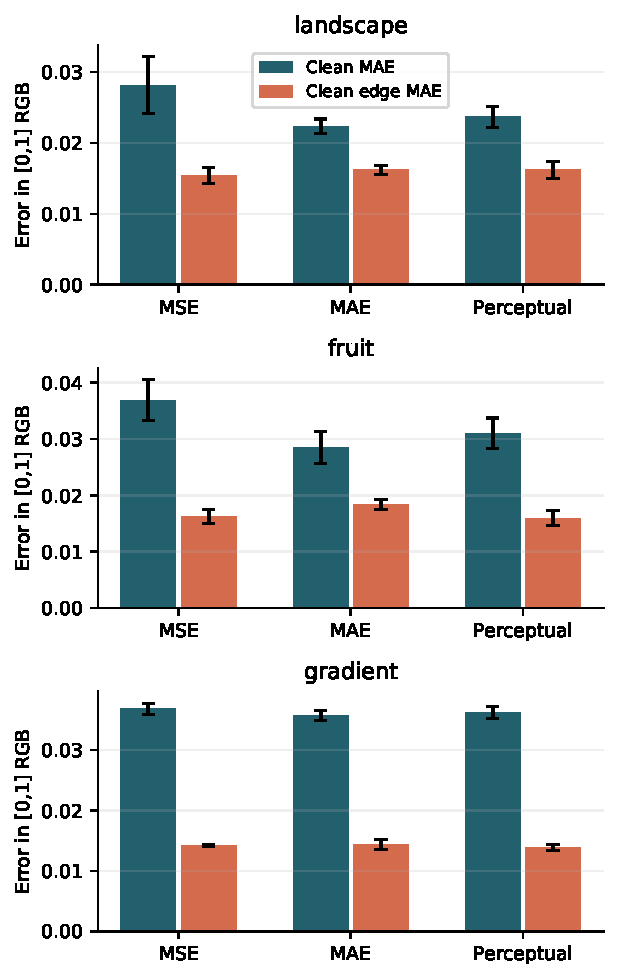
\includegraphics[width=\linewidth]{06/results/objectives.pdf}
\caption{ノイズ画像に学習した24三角形のclean MAEと輪郭MAE．目的関数と対応する色推定（MSEは平均値，その他は中央値）を組み合わせた設定の比較であり，損失関数だけの比較ではない．平均と標本標準偏差を示す．}
\label{fig:q06_objectives}
\end{figure}

\begin{figure}[t]
\centering
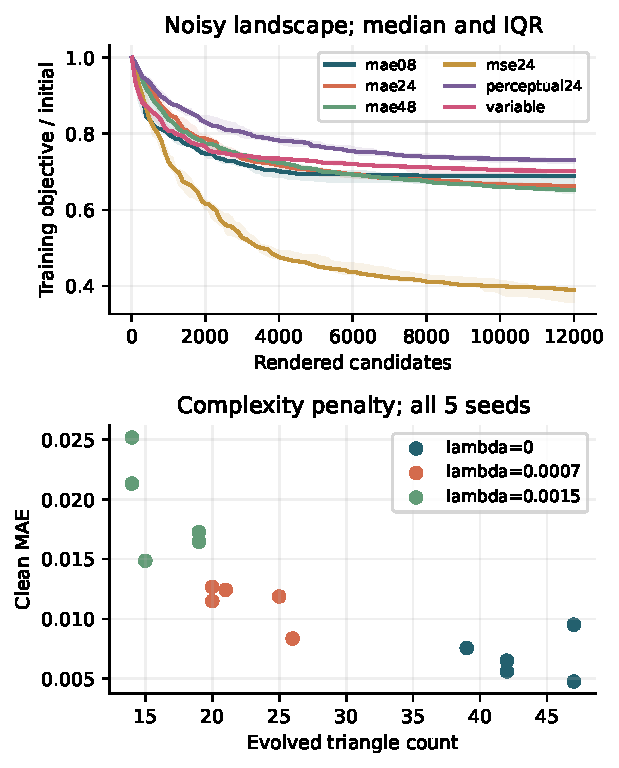
\includegraphics[width=\linewidth]{06/results/evolution_pareto.pdf}
\caption{上：ノイズを含む風景の探索推移（中央値と四分位範囲）．縦軸は各条件自身の初期目的値で割った比であり，異なる目的関数の絶対値を同一尺度として比較していない．下：ノイズなし風景の可変長版で，複雑さ罰則を変えた各seedの三角形数とMAE．}
\label{fig:q06_pareto}
\end{figure}

\subsection{考察と改善案}
三角形の枚数は一種の正則化として働く．少ない面しか使えないため，各画素に独立なノイズをそのまま記憶しにくい．他方，極端に少ない面では葉や雪の境界も消えてしまう．$\lambda n$の費用は，この複雑さと忠実さの選択を明示的に表している．本実験では少数の独立な探索seedしか扱っていないため，小さな平均差を統計的な一般則と断定しない．

適用範囲も限定される．ここで扱ったのは小さい合成画像3種類であり，自然写真，大きい解像度，半透明表現，多人数による主観評価は未検証である．特に滑らかな勾配を不透明な一定色の三角形で表すと，少数の面では色の段差が残る．対象の性質に合わせて表現自体を変えることも，探索方法を改良することと同程度に重要である．

知覚項については，人間が重要だと感じる境界と，単に数値的に強い局所差分を区別することが次の課題である．例えばノイズを抑えた複数解像度の輪郭，知覚色空間での色差，主対象に重みを付けるマスクを導入できる．ただし，目的項が増えるほど探索が難しくなるため，候補数一定の場合と計算時間一定の場合の両方で比較する必要がある．

人間の好みを直接扱うにはIECも有望である．例えば，誤差と三角形数のパレート前線上の候補を少数だけ提示し，「どちらが好ましいか」の対比較から選好モデルを作れば，単一のMAE値より感覚を反映できる可能性がある．その際は，評価者数，提示順のランダム化，疲労，個人差を記録すべきである．今回は人間の評価を実施していないため，IECによる改善や美的優越性は主張しない．

再現性のため，元画像生成コード，乱数seed，最終遺伝子，全試行の目的値と所要時間，収束履歴を保存した．表と図は同じJSONから再生成する．また，公開JSONからPNGとSVGを出力できる．SVGは連続座標を保つため，整数画素に丸めた評価用画像とは境界がわずかに異なる点をREADMEに明記した．

\repolink{06}
